
\documentclass[12pt,journal,compsoc]{IEEEtran}
\usepackage{array}
\usepackage{bytefield}
\usepackage{graphicx}
\usepackage{listings}
\usepackage{slashbox}
\usepackage{tikz}
\lstset{
frame=tb,
language=C,
aboveskip=3mm,
belowskip=3mm,
showstringspaces=false,
columns=flexible,
basicstyle={\small\ttfamily},
numbers=none,
breaklines=true,
breakatwhitespace=true,
tabsize=3
}
\hyphenation{op-tical net-works semi-conduc-tor}
\newcounter{mcount}
\setcounter{mcount}{0}
\begin{document}
\title{Reliable Multicast tool using UDP/IP}
\author{David Gong, Stephen Hamilton}% <-this % stops a space
\date{Sunday, September 21, 2014}
\IEEEtitleabstractindextext{%
\begin{abstract}
Our goal is to develop a multicast system capable of reliably sending packets in agreed order utilizing the UDP/IP protocol. In order to accomplish this task, we will implement a ring protocol where a token is passed in order to establish the control of sending packets. A node will only be able to send packets when the node is in possession of the token.
\end{abstract}
}
\maketitle
\section{Introduction}
\IEEEPARstart{T}{his} multicast ring protocol works by utilizing a token to control the flow of packets multicasted to all processes. There are three stages to this protocol. First is the startup which involves initializing the processes and determining the ring-path for the token.

The second stage is data transmission. Once the processes are initiated, the first process will generate the first token. If that machine has data to send, it will send data up to the maximum flow control value (which is pre-defined but also adapts as the program progresses). Once it has sent the data, it will send an updated token to the next machine. The next process then writes from its received data packets up to the min(token\_aru, previous\_token\_aru). It resends any requests contained in the rtr and it sends the packets it needs to send, updates the token sequence number, rtr, an finally sends the token. And so the cycle repeats. Due to the potential for loss over UDP, this protocol has an additional field on the token called loss\_level which determines the number of times a token is sent per attempt from one process to another. This protocol will attemp to adapt the loss\_level by detecting when a token is lost. The intent is to increase the reliability of the token by sending it multiple times.

Finally, because properly ending is provably unsolvable, we adopt the method of termination that relaxes the requirement for theoretical, finite termination, but in practical settings will work by drastically reducing the chance of failure after every attempt further.
\section{Design}
\subsection{Assumptions}
Before delving into the specifics of our protocol, there are a few assumptions on which the success of our protocol depends.
\begin{itemize}
\item Machine ids will be in sequential and continuous order up to the maximum number of machines (10).
\end{itemize}
With these assumptions, we can describe a successful multicast protocol for agreed data ordering over UDP.
\subsection{Token Design}
\begin{lstlisting}
// Structure of token.
int type;//Type of packet
int sequence;//Sequence of last message
int aru;//Sequence of all rcv up to
int fcc;//Flow control/Max send size
int rtr[MAX_RTR];//Array of Retransmit requests
int rtrcount;//Number of entries in rtr array
int loss_level;//Increases on token regeneration
int nodata[10];//Process completion flag
int round;//Number of ring traversals
int aru_lowered_by;//Flag for lowering the aru
\end{lstlisting}
The token contains all the necessary data needed to maintain the flow of the protocol. It holds the global maximum sequence number so that senders know what the sequence of the most recently sent packet is. The aru on the token helps with necessary protocol semantics. The fcc aids in controlling data flow. The rtr is used by machines to make requests for missing packets. And nodata is the field used to determine the protocol's termination. Other fields are kept in order to optimize the protocol in the way we thought best.

\subsection{Data Packet Design}
The data structure we plan to implement is an array of packets. This list will contain all the sent packets that are greater than min(token.aru, previous token.aru). It will be implemented in a struct as follows:
\begin{lstlisting}
struct packet_structure {
int type;//Type of packet
int sequence;//Sequence of packet
int received;//Flag for when globally received
int machine_index;//Index of packet's sender
int random_number;//Data
char data[packet_size];//Contents
}
\end{lstlisting}
The packet structure contains the overall token sequence, whether or not the packet was received, the machine\_index of the sender, the random number, the 1200 additional payload bytes, along with the pointer to the next packet.
\subsection{Data Structure}
This protocol uses one main data structure per machine in order to control the information flow for each machine.

\begin{figure}[h]
\centering
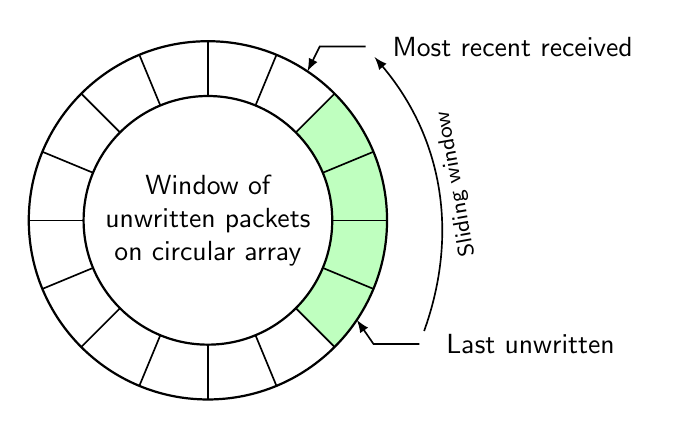
\begin{tikzpicture}[>=latex,font=\sffamily,semithick,scale=1.75]
    \fill [green!25] (0,0) -- (45:1.3) arc [end angle=-45, start angle=45, radius=1.3] -- cycle;
    \draw [thick] (0,0) circle (1.3);
    \foreach \angle in {90,67.5,...,-67.5}
        \draw (\angle:1.3) -- (\angle-180:1.3);
    \node [circle,thick,fill=white,draw=black,align=center,minimum size=3cm] at (0,0) {Window of\\unwritten packets\\on circular array};
    \draw [<-] (56.25:1.3) -- (57.25:1.5) -- +(.333,0)
        node [right,inner xsep=.333cm] (Head) {Most recent received};
    \draw [<-] (-33.75:1.3) -- (-36.75:1.5) -- +(.333,0)
        node [right,inner xsep=.333cm] (Tail) {Last unwritten};
    \draw [->,shorten >=5pt,shorten <=5pt] (Tail.west) to [bend right] 
        node [midway,sloped, below,allow upside down] {\footnotesize Sliding window}
    (Head.west);
\end{tikzpicture}
\caption{Representation of the circular array used to store unwritten packets.}
\end{figure}

Each machine has a circular array (as in Figure 1). The array holds all of the received packets that haven't been written. The packets can only be written if their sequence value is lower than the minimum of the previous token aru and the current token aru. After the packet is written, the slot in the array is freed and the window can progress. We need not worry about filling and writing over the maximum window size because we have the fcc to control data flow.

\subsection{State Machine}
\begin{figure}[h]
\centering
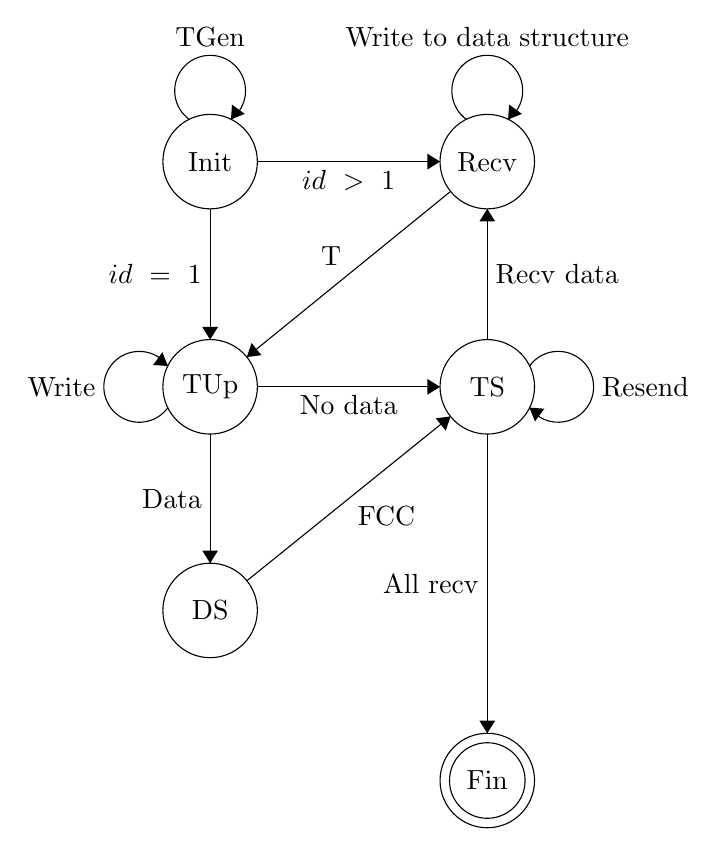
\begin{tikzpicture}[scale=0.2]
\tikzstyle{every node}+=[inner sep=0pt]
\draw [black] (21.4,-11.2) circle (3);
\draw (21.4,-11.2) node {$\mathrm{Init}$};
\draw [black] (21.4,-25.5) circle (3);
\draw (21.4,-25.5) node {$\mathrm{TUp}$};
\draw [black] (39,-11.2) circle (3);
\draw (39,-11.2) node {$\mathrm{Recv}$};
\draw [black] (39,-25.5) circle (3);
\draw (39,-25.5) node {$\mathrm{TS}$};
\draw [black] (21.4,-39.7) circle (3);
\draw (21.4,-39.7) node {$\mathrm{DS}$};
\draw [black] (39,-50.5) circle (3);
\draw (39,-50.5) node {$\mathrm{Fin}$};
\draw [black] (39,-50.5) circle (2.4);
\draw [black] (18.72,-26.823) arc (-36:-324:2.25);
\draw (14.15,-25.5) node [left] {$\mathrm{Write}$};
\fill [black] (18.72,-24.18) -- (18.37,-23.3) -- (17.78,-24.11);
\draw [black] (21.4,-28.5) -- (21.4,-36.7);
\fill [black] (21.4,-36.7) -- (21.9,-35.9) -- (20.9,-35.9);
\draw (20.9,-32.6) node [left] {$\mathrm{Data}$};
\draw [black] (24.4,-25.5) -- (36,-25.5);
\fill [black] (36,-25.5) -- (35.2,-25) -- (35.2,-26);
\draw (30.2,-26) node [below] {$\mathrm{No\ data}$};
\draw [black] (23.73,-37.82) -- (36.67,-27.38);
\fill [black] (36.67,-27.38) -- (35.73,-27.5) -- (36.36,-28.28);
\draw (32.6,-33.09) node [below] {$\mathrm{FCC}$};
\draw [black] (39,-22.5) -- (39,-14.2);
\fill [black] (39,-14.2) -- (38.5,-15) -- (39.5,-15);
\draw (39.5,-18.35) node [right] {$\mathrm{Recv\ data}$};
\draw [black] (36.67,-13.09) -- (23.73,-23.61);
\fill [black] (23.73,-23.61) -- (24.66,-23.49) -- (24.03,-22.72);
\draw (29.08,-17.86) node [above] {$\mathrm{T}$};
\draw [black] (21.4,-14.2) -- (21.4,-22.5);
\fill [black] (21.4,-22.5) -- (21.9,-21.7) -- (20.9,-21.7);
\draw (20.9,-18.35) node [left] {$id\mbox{ }=\mbox{ }1$};
\draw [black] (24.4,-11.2) -- (36,-11.2);
\fill [black] (36,-11.2) -- (35.2,-10.7) -- (35.2,-11.7);
\draw (30.2,-11.7) node [below] {$id\mbox{ }>\mbox{ }1$};
\draw [black] (37.677,-8.52) arc (234:-54:2.25);
\draw (39,-3.95) node [above] {$\mathrm{Write\ to\ data\ structure}$};
\fill [black] (40.32,-8.52) -- (41.2,-8.17) -- (40.39,-7.58);
\draw [black] (41.68,-24.177) arc (144:-144:2.25);
\draw (46.25,-25.5) node [right] {$\mathrm{Resend}$};
\fill [black] (41.68,-26.82) -- (42.03,-27.7) -- (42.62,-26.89);
\draw [black] (20.077,-8.52) arc (234:-54:2.25);
\draw (21.4,-3.95) node [above] {$\mathrm{TGen}$};
\fill [black] (22.72,-8.52) -- (23.6,-8.17) -- (22.79,-7.58);
\draw [black] (39,-28.5) -- (39,-47.5);
\fill [black] (39,-47.5) -- (39.5,-46.7) -- (38.5,-46.7);
\draw (38.5,-38) node [left] {$\mathrm{All\ recv}$};
\end{tikzpicture}
\caption{A general state machine for the program from the perspective of a machine. T is for token, D is for data, S is for send, Up is for update.}
\end{figure}

\subsection{Algorithm}
We dedicate a section to explaining the details of the protocol. As stated before, the protocal is split into three main parts: startup, message transmission, termination. The general flow of our protocol is shown in Figure 1.

The startup is difficult because we must find a way to successfully establish the ring through which the token is passed (using unicast). Our approach to this is a simple ack routine. Every machine starts out by multicasting its own information so that everyone (ncluding the target) receives the information. In the meantime, every machine also filters through the received packets, looking for its target (the machine with the next sequential ID). Once it successfully receives the information, it sends a message to machine 1 (who is essentially the controller). If a machine does not receive its neighbor, it sends out a request for machine ids.  For machines who already know their neighbor, they will respond to this request with their machine id.  Machine 1 will not create the token until all machines are done, therefore the transmission process will not start until everyone is ready to receive the token. Once all acks are received, the process starts with machine 1 sending data and when complete it sends the token to process 2.

The transmission proceeds as discussed in the introduction essentially covers everything. A note is that flow control is determined by how often various limits are reached. For example, if the rtr ever reaches a state of being completely full, then we lower the fcc meaning that people must send less (giving more opportunitites time for the machines to catch up).

We also built in an adaptive part of token recovery.  Once our loss level exceeds 3 (it increases upon each token loss), the token will be sent three times between each process.  In practice, we found that adding this adaptation significantly reduced the number of token losses, giving us better finish times overall.  This tuning could be further defined to run over time so that if token loss stops occurring (over a pre-defined number of rounds), the loss level could be reduced and eventually processes will send one token instead of three.  It could also be expanded to send a varying number of tokens depending on the loss detected.  

Finally, termination is done when the array in the token reflects that all processes are done sending data (a 1 for each process), and the token aru, prior token aru, and token sequence are all the same.  This means there is no data left to send, and everyone has received all data sent.  Once this is true, each process sends a mass of tokens (100) before finaly closing. That way the probability of none of them being received is close to 0 in a practical setting.

\section{Results}
\begin{table}[h]
\begin{center}
\begin{tabular}{|r|r|r|r|r|r|r|}\hline
\backslashbox{Trial}{Loss} & 0\% & 1\% & 2\% & 5\% & 10\% & 20\%\\\hline
1 & 8.00 & 8.63 & 8.60 & 10.24 & 11.98 & 17.79\\\hline
2 & 7.99 & 8.58 & 9.06 & 10.22 & 11.92 & 18.70\\\hline
3 & 7.96 & 8.50 & 8.95 & 10.21 & 11.97 & 17.89\\\hline
4 & 7.97 & 8.64 & 9.08 & 10.19 & 11.99 & 16.49\\\hline
5 & 8.08 & 8.54 & 8.98 & 10.18 & 11.98 & 15.75\\\hline
\end{tabular}
\end{center}
\caption{5 time trials in seconds, each of varying \% packet loss.}
\end{table}
\begin{table}[h]
\begin{center}
\begin{tabular}{|r|r|}\hline
\% Loss & Average time (s)\\\hline
0 & 8.00\\\hline
1 & 8.58\\\hline
2 & 8.93\\\hline
5 & 10.21\\\hline
10 & 11.97\\\hline
20 & 17.32\\\hline
\end{tabular}
\end{center}
\caption{Average times for each level of packet loss.}
\end{table}
Table 1 and Table 2 are the results of the benchmarks we ran on our protocol. We ran our protocol with simulations of loss at 0\%, 1\%, 2\%, 5\%, 10\%, and 20\%, 5 times each. The average of those times is shown in Table 2.

\begin{figure}[h]
\includegraphics[width=\linewidth]{Multicast1.png}
\caption{Graphical interpretation of results}
\end{figure}
This is the data of Table 2 displayed as a graph.

\section{Conclusion}
Our results are fairly consistent with our expectation. The graph displays our expectation that as loss grows the length of time to finish increases.  We also see that the program's degredation seems close to linear, which would be ideal. Our goal was was to get the slope as flat as possible. We realized that losing the token takes a huge toll on running time since a timeout will occur before processes can send data. However, this data is evidence that our protocol responded fairly well with token loss. There is still room for improvement as our transmission time slightly more than doubles when comparing 0\% loss to 20\% loss.

We send a total of 600,000 packets, and we calculate each packet size to be 1200 bytes + 6 int fields (24 bytes) + 2 bytes UDP header = 1226 bytes.  This is about 5612 Mbits. Under 0\% loss it takes around 8 seconds so the transfer rate is around 701 Mib/s. This degrades as loss grows -- at 20\%, the transfer rate is around 332 Mib/s.

\section{Discussion}
The token ring protocol we implemented transfers its messages in agreed order and can handle significant loss. Some improvements we could make to our protocol would be to take the next step and do the data transmission after updating/sending the token (advanced token ring protocol). But in general, the main place we can make improvements in is tweaking the data structure size, modifying the retransmission request size allowance, and playing with the method of evolution of the fcc while the protocol runs. These small changes could potentially have a large affect on preventing the protocol from hitting periods of lag, for example, when one process gets too far behind the others.

We also had an interesting observation that could lead to tuning our protocol for better adaptation.  At 10\% loss, there was a high probability we would hit our limit of too many outstanding packets (our data structure was full), and machines would have to wait another round to send packets.  This did not occur at 20\% loss, which was due to the fact that the RTR limit was reached early on, and the FCC was reduced so that the too many outstanding packet condition was never reached.  Further testing of reducing the FCC when the oustanding packet condition was reached may yield faster times with the 10\% loss rate.  
\end{document}
